%!TEX root = ../thesis.tex
\chapter{Conclusions}
\label{conclusions}

After having explained how this solution has been implemented, I would like to draw the conclusions on the project, internship experience and knowledge acquired.

\section{Objectives achievement}
	Even thought the original objectives have changes during the internship, the software's documentation and the blogs presented contained the correct answers in order to correctly configure the software.\\
	Here is a list of the requirements and their status at the end of the project:
	\begin{itemize}
		\item \underline{\textit{O01}}: ACHIEVED
		\item \underline{\textit{O02}}: ACHIEVED
		\item \underline{\textit{O03}}: ACHIEVED
		\item \underline{\textit{O04}}: ACHIEVED
		\item \underline{\textit{O05}}: ACHIEVED
		\item \underline{\textit{D01}}: NOT IMPLEMENTED
		\item \underline{\textit{D02}}: NOT IMPLEMENTED
		\item \underline{\textit{D03}}: ACHIEVED
		\item \underline{\textit{D04}}: NOT IMPLEMENTED
		\item \underline{\textit{D05}}: ACHIEVED
		\item \underline{\textit{D06}}: ACHIEVED
		\item \underline{\textit{F01}}: NOT IMPLEMENTED
		\item \underline{\textit{F02}}: NOT IMPLEMENTED
	\end{itemize} 
	Note that the ones with \Quote{NOT IMPLEMENTED} status is because of internal rules that would not allow interns to interact with the production environment.\\
	Although these have not been achieved, the knowledge on how to implement them has been acquired since their description is contained in the documentation that has been left in Athonet.

\section{Improvement and future implementations}
	As many other projects there are many improvements that can applied.
	To complete the project presented in this thesis I would move it into a production environment and migrate the data from the Redmine instance.
	To have a better and more stable environment thought, there are various improvements that could be made.
	The first and most important one, in my personal opinion, would be separating the database from the Virtual Machine that hosts the software.
	This would bring advantages like: 
	\begin{itemize}
		\item the machine with Jira and Confluence would be less stressed since it would not have so many reads and writes per disk
		\item the database could be stores in a single machine (or multiple ones) with dedicated disks arranged in a redundant way which adds a layer of security, in a disaster recovery plan, over regular backups
		\item maintenance to either one of the machines would be easier and would impact less the company's work
		\item etc.
	\end{itemize}
	Another important improvement would be separating the Confluence instance from the Jira one and, instead of having them running on a dedicated Virtual Machine each, creating a Docker \cite{dock} \gls{container}\glsadd{Container} so that they would be easier to handle (copy, migrate, update).
	\begin{figure}[H]
		\centering
		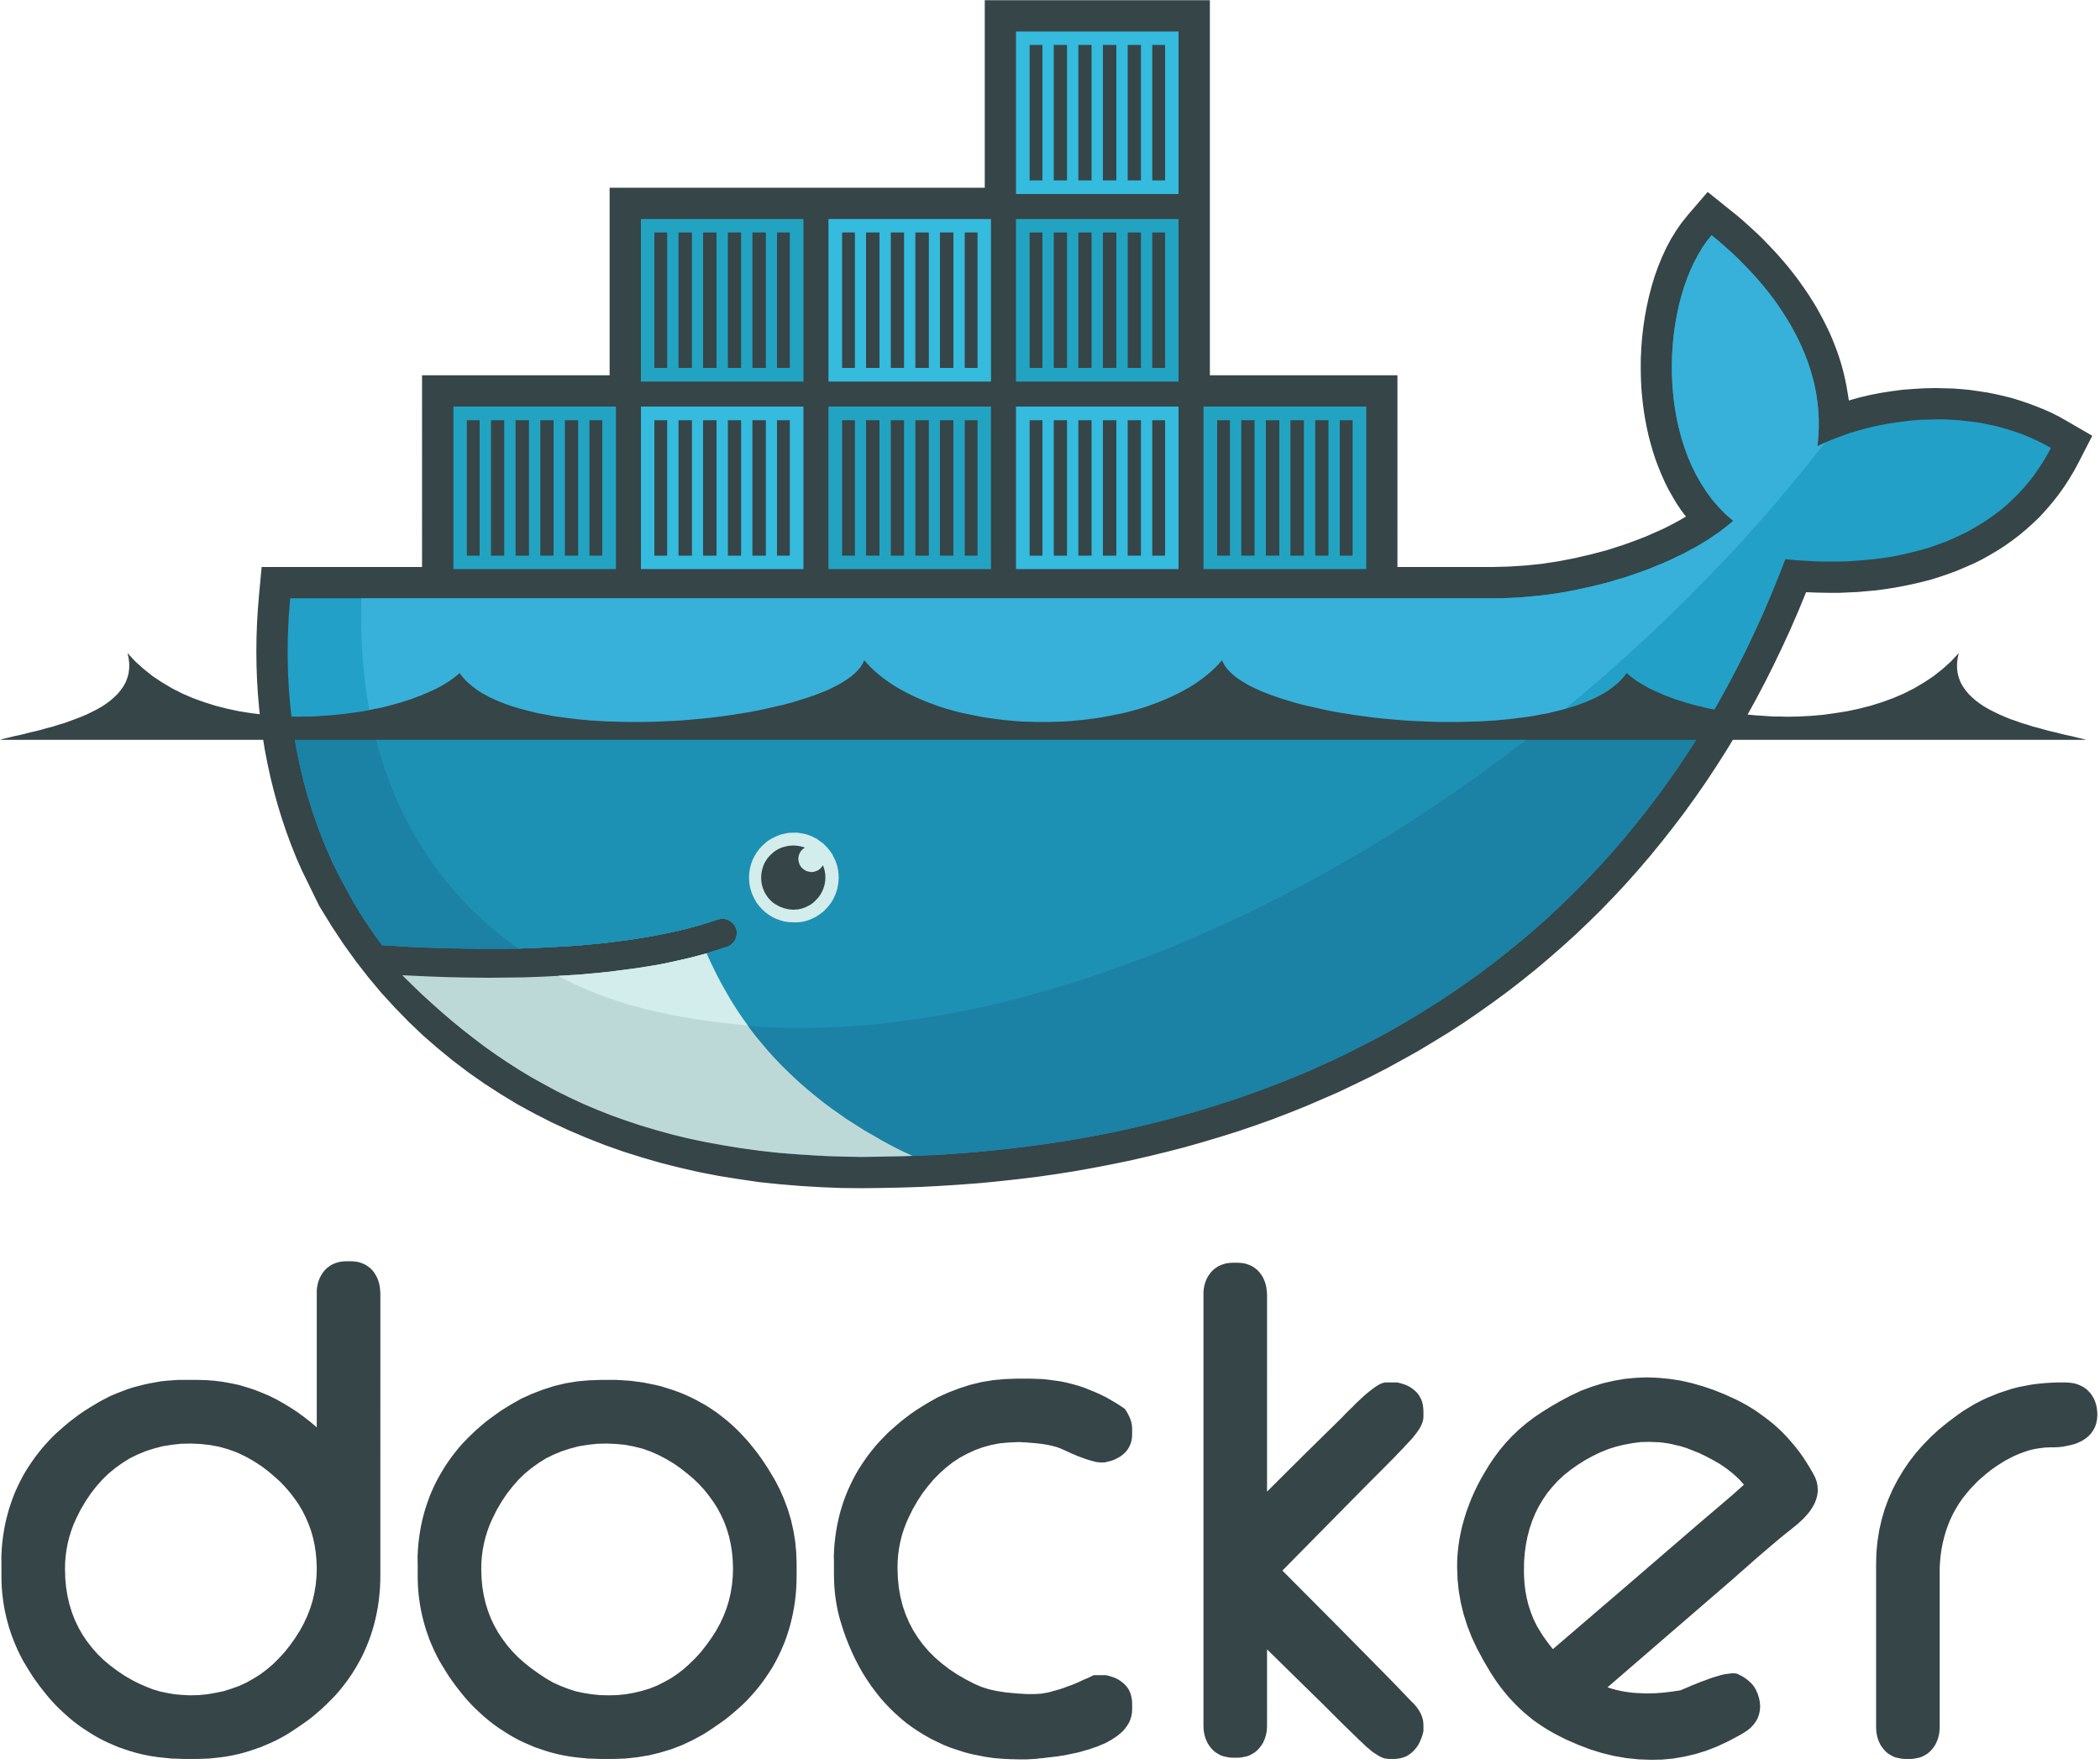
\includegraphics[width=.4\textwidth]{resources/docker}\\
		\caption{Docker logo}
	\end{figure}
	The use of containers would also allow a better usage of the host machine's resources like memory and CPU power by sharing them.
	These would otherwise be split and left unused by the VMs.
	This kind of improvements should be implemented when planning the migration of the services in a production environment.\\
	Other future improvements can be installing plugins that would allow connectivity with the Microsoft Office suite allowing employees to produce documents and reports without learning how to do it in Confluence and just uploading them.

\section{What I have learned}
	During this internship I had the possibility to better understand the hierarchy of a company, an argument well introduced in the Software Engineering (SWE) course.
	In Athonet I had the possibility to see this first hand and to interact with people on more levels of responsibility, from the CTO, to the product owner to the managers of verification and development teams.\\
	About the tools, it is important to know how to use software like this not only for tracking the status of issues but on how to see other information about them as well.
	This kind of tools are are found in many IT companies, small or big, since they ease not only the work of keeping track of issues but the documentation of meeting notes, internal documents, release changelogs and many other features as well.\\
	In a growing company like Athonet it is useful to set some boundaries, not only for lower level employees like developers, but for the management as well.